\section{Các kỹ thuật Word Embedding}
\label{sec:word-embedding-in-details}
Hầu hết những giải thuật Machine Learning, đặc biệt là những giải thuật sử dụng mạng nơ-ron như MLP, Deep Learning không làm việc hiểu quả trên dữ liệu văn bản. Word Embedding là một trong những là kĩ thuật được sử dụng trong xử lý ngôn ngữ tự nhiên nhằm số hoá một từ ở dạng văn bản mà con người hiểu, sang dạng cho phép máy tính có thể tính toán và xử lý được. 

Word embedding được sử dụng rộng rãi và phổ biến trong những dự án xử lý ngôn ngữ tự nhiên không chỉ vì khả năng biểu diễn văn bản dưới dạng số, mà kĩ thuật này còn cho phép nhúng (embedding) ngữ nghĩa của từ trong văn bản vào định dạng số mà máy tính có thể hiểu và xử lý hiệu quả.

Từ khi khái niệm word embedding ra đời, đã có rất nhiều giải thuật được trình bày như word2vec, GolVe, ELMO, BERT, v.v. Tuy nhiên một giải thuật Word embedding cần phải thoả mãn 2 yêu cầu dưới đây:

\begin{itemize}
    \item Tồn tại một và chỉ một cách biểu diễn cho một từ. Nghĩa là hai từ khác nhau sẽ được số hoá thành hai dạng biểu diễn khác nhau.
    
    \item Hai từ có ngữ nghĩa tương tự nhau, khoảng cách cũng sẽ gần nhau sau khi được biểu diễn sang không gian mới.
\end{itemize}


\subsection{Biểu diễn từ bằng one-hot vector}
\label{one-hot-vector-in-details}

Trước khi Word embedding ra đời, kĩ thuật được sử dụng phổ biến để số hoá một từ là sử dụng one-hot vector. Kĩ thuật này được áp dụng trong các mô hình học máy cổ điển trong giai đoạn tiền xử lý, nhằm biến đổi những dữ diệu dạng categorical sang numerical. Từ đó giúp máy tính có thể tính toán và xử lý được.

One-hot vector là một vector chứa dữ liệu nhị phân (0 và 1), tuy nhiên chỉ có một chiều trong vector được kích hoạt mang giá trị 1, toàn bộ những chiều còn lại đều mang giá trị 0. One-hot encoding là kĩ thuật biểu diễn một tập các giá trị rời rạc sang một tập one-hot vector. Để hiểu rõ hơn, xem xét ví dụ dưới đây.

Danh sách nhà mạng viễn thông ở Việt Nam là một tập hợp các giá trị rời rạc bao gồm: Viettel, Mobifone, Vinaphone, Sphone, Beeline. Sử dụng kĩ thuật one-hot vector, chúng ta có thể biểu diễn giá trị Mobifone bằng một vector trong hình \ref{fig:mobifone-onthot}.

\begin{figure}[h!]
\begin{center}
	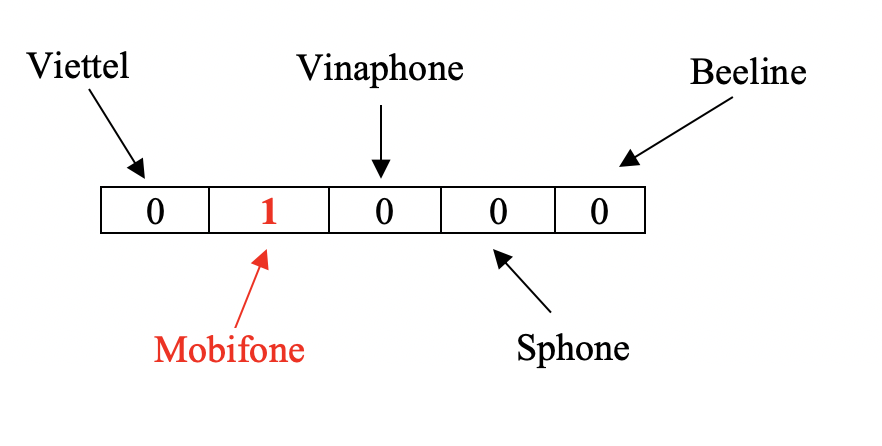
\includegraphics[width=1.0\textwidth]{chapter04/figure/mobifone-onehot.png}
	\caption{Biểu diễn Mobifone bằng one-hot vector.}
	\label{fig:mobifone-onthot}
\end{center}
\end{figure}

Vector này có 5 chiều tương đương với 5 nhà mạng chúng ta có. Trong đó tại chiều thứ 2, tương ứng với vị trí của Mobifone trong danh sách nhà mạng, mang giá trị 1, những chiều còn lại mạng giá trị không. Tự tự, chúng ta có thể biểu diễn các nhà mạng khác bằng các vector one-hot được trình bày trong bảng \ref{table:one-hot-vector-example}.

\begin{table}[h!]
    \centering
    \begin{tabular}{ |c|c|c|c|c|c| } 
    \hline
         & Viettel & Mobifone & Vinaphone & SPhone & Beeline \\
    \hline
        Viettel & 1 & 0 & 0 & 0 & 0 \\
        Mobifone & 0 & 1 & 0 & 0 & 0\\
        Vinaphone & 0 & 0 & 1 & 0 & 0\\
        SPhone & 0 & 0 & 0 & 1 & 0\\
        Beeline & 0 & 0 & 0 & 0 & 1 \\
    \hline
    \end{tabular}
    \caption{Sử dụng one-hot vector để biểu diễn các nhà mạng ở Việt Nam}
    \label{table:one-hot-vector-example}
\end{table}

Chúng ta có thể dễ dàng nhận thấy, tập hợp từ trong văn bản cũng thuộc miền giá trị rời rạc. Do đó, kĩ thuật one-hot encoding có thể sử dụng nhằm biểu diễn một từ sang dạng one-hot vector.

Xem xét các câu sau đây (sau khi tokenize):
\begin{itemize}
    \item Hôm\_qua tôi đi học
    \item Hôm\_nay tôi cũng đi học
    \item Ngày\_mai tôi không đi học
\end{itemize}

Tập từ điển của chúng ta có 8 từ: "Hôm\_qua", "Hôm\_nay", "Ngày\_mai", "Tôi", "Đi", "Học", "Cũng", "Không". 

Để biểu diễn sang dạng số, chúng ta sử dụng one-hot vector có 8 chiều. Tám tương ưng ứng với số từ trong từ điển. Mở rộng ra, khi từ điển chúng ta có n từ, chúng ta biến đổi mỗi từ sang one-hot vector có n chiều. Đa phần các chiều của vector mang giá trị 0, chỉ duy nhất ở chiều tương ứng với vị trí của từ trong từ điển được kích hoạt mạng giá trị 1. Bảng \ref{table:one-hot-vector-from-dict} thể hiện việc chuyển đổi từ sang one-hot vector.

\begin{table}[h!]
    \centering
    \begin{tabular}{ |c|c|c|c|c|c|c|c|c| } 
    \hline
         & Hôm\_qua & Hôm\_nay & Ngày\_mai & Tôi & Đi & Học & Cũng & Không \\
    \hline
        Hôm\_qua & 1 & 0 & 0 & 0 & 0 & 0 & 0 & 0 \\
        Hôm\_nay & 0 & 1 & 0 & 0 & 0 & 0 & 0 & 0\\
        Ngày\_mai & 0 & 0 & 1 & 0 & 0 & 0 & 0 & 0\\
        Tôi & 0 & 0 & 0 & 1 & 0 & 0 & 0 & 0\\
        Đi & 0 & 0 & 0 & 0 & 1 & 0 & 0 & 0\\
        Học & 0 & 0 & 0 & 0 & 0 & 1 & 0 & 0\\
        Cũng & 0 & 0 & 0 & 0 & 0 & 0 & 1 & 0\\
        Không & 0 & 0 & 0 & 0 & 0 & 0 & 0 & 1 \\
    \hline
    \end{tabular}
    \caption{Sử dụng one-hot vector để biểu diễn các từ trong từ điển.}
    \label{table:one-hot-vector-from-dict}
\end{table}

Dựa vào kĩ thuật One-hot encoding, chúng ta đã có thể biểu diễn bất kì từ nào sang dạng số mà máy tính có thể xử lý. Rất nhiều mô hình xử lý ngôn ngữ tự nhiên và học máy đã sử dụng kĩ thuật này và mang lại hiệu quả khả quan, đặc biệt khi số lượng từ trong từ điển tương đối nhỏ. Tuy kĩ thuật này đã đảm bảo được yêu cầu biểu diễn hai từ khác nhau với hai vector khác nhau, nó vẫn mang nhiều khuyết điểm cần được cải tiến:

\begin{itemize}
    \item Giới hạn khả năng tính toán của máy tính: Hầu hết các chiều của one-hot vector mang giá trị 0, và nhiều mô hình học máy không làm việc hiệu quả trên vector có số chiều lớn (high dimensional vector) và “thưa” (sparse vector).
    
    \item Overfitting khi số lượng từ trong từ điển tăng: Với kĩ thuật này, mỗi khi chúng ta gia tăng số lượng từ trong từ điển lên n, số chiều của one-hot vector cũng tăng tương ứng lên n. Bởi vì số chiều của vector tương ứng với số lượng từ ta có trong từ điển. Trong ví dụ trên chúng ta chỉ có 8 từ trong từ điển, nhưng trong thực tế số từ trong từ điển là rất lớn, có thể đến vài ngàn, chục ngàn từ. Càng nhiều từ, càng nhiều thông số (parameter) mà mô hình học máy cần phải học. Càng nhiều thông số, chúng ta lại cần càng nhiều dữ liệu huấn luyện (training dataset) để xây dựng mô hình tốt, và không bị overfitting.
    
    \item Thiếu khả năng tổng quát hoá: Qua quá trình tiến hoá của con người, ngôn ngữ được sinh ra và phát triển theo thời gian. Khi nhìn vào một từ, chúng ta không chỉ biết ý nghĩa của mỗi từ đó mà còn hiểu được sự liên kết với những từ khác, và có khả năng tổng quát hoá ý nghĩa của một nhóm các từ liên quan. Nhờ khả năng tổng quá hoá, chúng ta có thể rút ngắn thời gian học một kiến thức mới. Ví dụ, chúng ta biết được mèo biết leo cây và ăn thịt, trong khi đó hổ và báo cũng tương tự như mèo (tổng quá hoá), nhờ vậy chúng ta có thể dự đoán được hổ vào báo cũng có thể leo cây và ăn thịt.
    
    Khi xây dựng một mô hình học máy, chúng ta muốn mô hình cũng có khả năng tổng quát hoá như chúng ta nhằm rút ngắn thời gian huấn luyện. Quay lại ví dụ trên, khi mô hình đang được huấn luyện trên dữ liệu đầu vào là “mèo”, chúng ta có dữ liệu đầu vào mới là “hổ”. Nếu hiểu được “mèo” và “hổ” tương tự nhau, mô hình không cần học “hổ” từ đầu, thay vào đó mô hình có thể sử dụng lại những thông số (parameter) được huấn luyện với đầu vào là “mèo”. Từ đó rút ngắn thời gian và lượng dữ liệu để huấn luyện mô hình. 
    
    Với kĩ thuật one-hot encoding, mỗi từ được biểu diễn thành một vector riêng lẽ, và khoảng cách giữa các vector đều bằng nhau và bằng sqrt(2). Do đó, mô hình không thể sử dụng lại những “kiến thức” đã được huấn luyện cho những từ liên quan với nhau về mặt ngữ nghĩa.

\end{itemize}

\subsection{Kỹ thuật Auto-Encoder để thu giảm số chiều}
\subsubsection{Giới thiệu}

Auto-Encoder là mô hình mạng nơ-ron, được huấn luyện dựa trên cơ chế học không giám sát (unsupervised learning), nhằm biểu diễn dữ liệu đầu vào ở dạng vector nhiều chiều (high-dimensonal vector) bằng một vector có số chiều nhỏ hơn (low-demensial vector). Mô hình này được sử dụng trong kĩ thuật dữ liệu (data engineering) cho phép thu giảm số chiều của dữ liệu đầu vào, nhằm giúp trực quan hoá dữ liệu; tăng khả năng tính toán của máy tính, giảm số lượng thông số của mô hình (parameter) từ đó rút ngắn thời gian huấn luyện; v.v. 

Mô hình Auto-Encoder hoạt động dựa trên cơ chế compress và reconstruct. Theo đó, mô hình phải học cách biểu diễn dữ liệu đầu vào với một lượng thông tin ít hơn (compress), sao cho nó vẫn có thể tái tạo lại được dữ liệu đầu vào dựa trên lượng thông tin đó (reconstruct). Một cách hiểu đơn giản là mô hình hoạt động tương tự như cơ chế nén và giải nén file của WinRar. Mô hình được phân loại trong mô hình học không giám sát (unsupervised learning) bởi vì chúng ta không cần chuẩn bị nhãn (ground-truth hoặc label) để huấn luyện mô hình. Nó sử dụng chính dữ liệu đầu vào làm nhãn, vì mục đính của mô hình là học để tái tạo lại dữ liệu ban đầu.

\subsubsection{Kiến trúc mô hình Auto-Encoder}

\begin{figure}[h!]
\begin{center}
	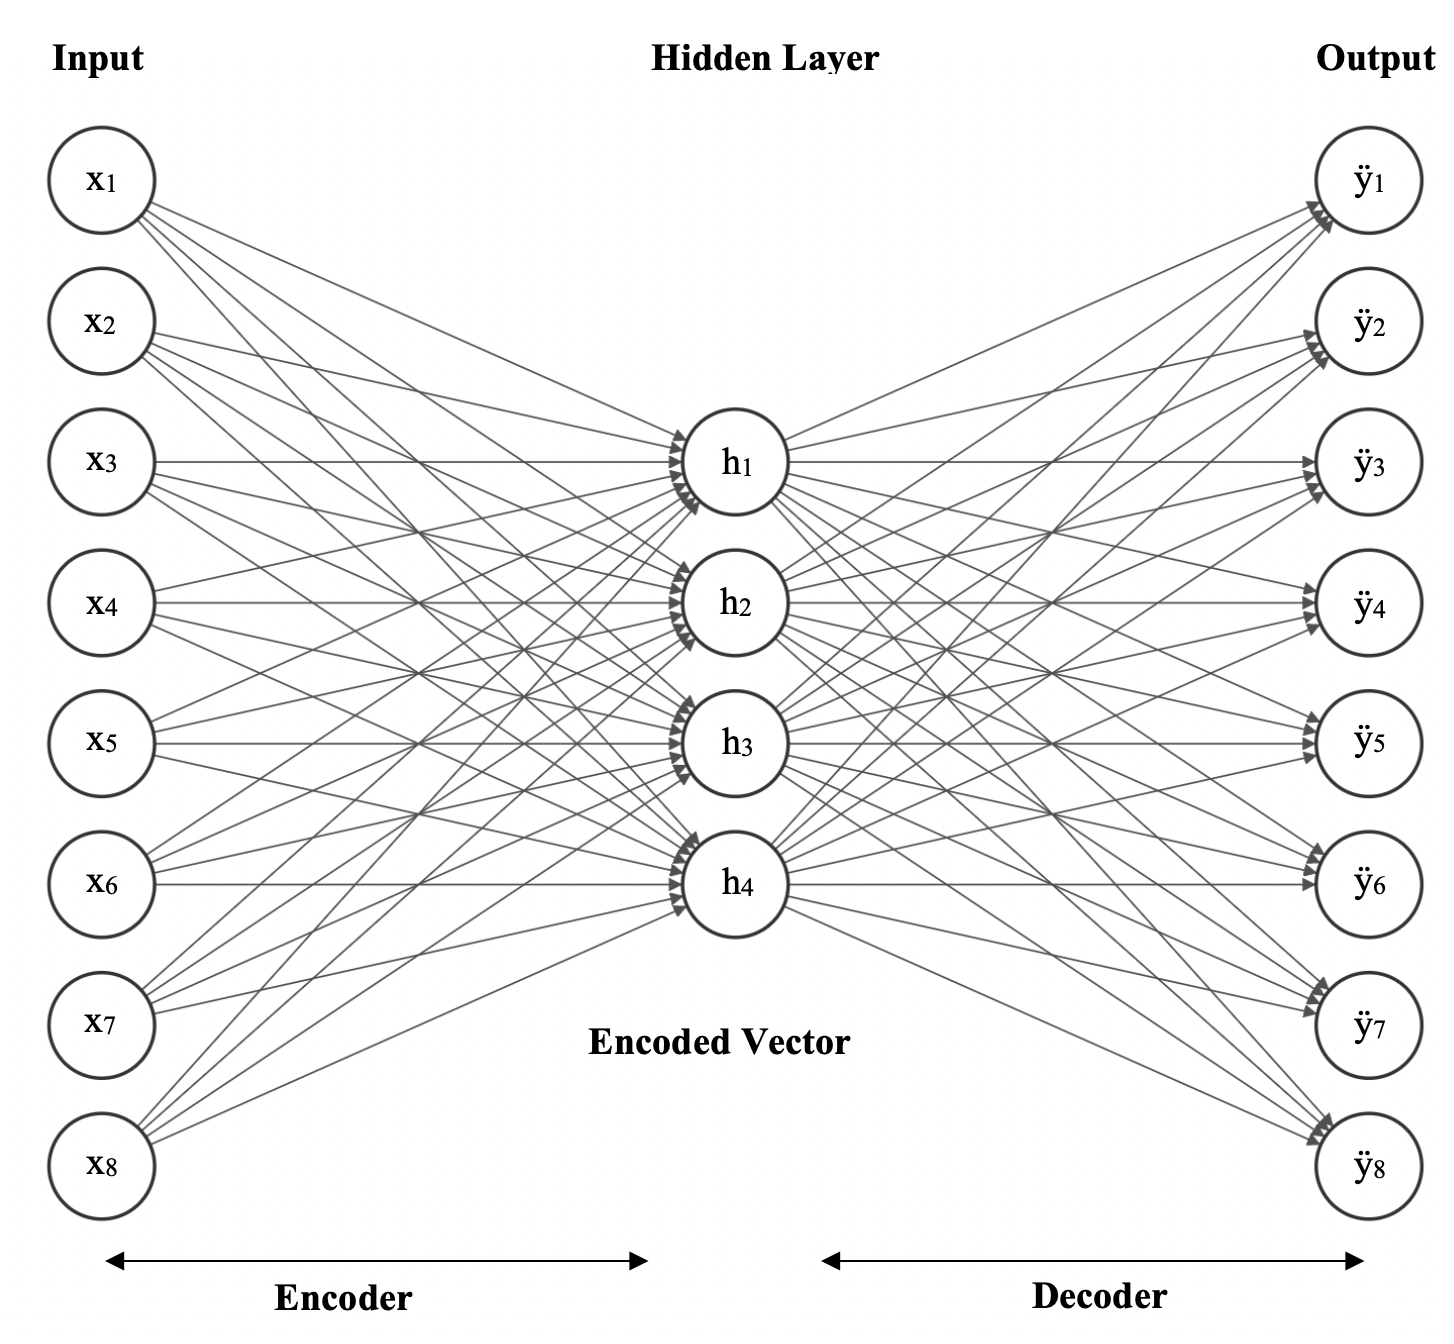
\includegraphics[width=1.0\textwidth]{chapter04/figure/auto-encoder-architecture.png}
	\caption{Mô hình Auto-Encoder sử dụng mạng nơ-ron 3 lớp.}
	\label{fig:auto-encoder-architecture}
\end{center}
\end{figure}

Kiến trúc mô hình Auto-Encoder là một mạng nơ-ron 3 lớp như hình \ref{fig:auto-encoder-architecture}. Trong đó hidden layer có số nút nhỏ hơn rất nhiều so với số nút ở Input và Output. Auto-Encoder bao gồm các thành phần quan trọng sau:

\begin{itemize}
    \item Encoder: là một ma trận Nxk, trong đó N là số chiều của vector đầu vào, k là số nút của hidden layer. Để mô hình  học được cách biểu vector đầu vào bằng một vector có số chiều nhỏ hơn, mô hình được thiết kế với số nút ở hidden layer nhỏ hơn so với số nút ở lớp Input và Output (k << N). Ma trận làm nhiệm vụ compress dữ liệu đầu vào ở không gian nhiều chiều N (high-dimensional space) sang không gian có số chiều nhỏ hơn k (low-dimensional space). Dữ liệu đầu vào sau khi đi qua ma trận Encoder, chúng ta nhận được một vector có số chiều là k, được gọi là encoded vector.
    \item Decoder: ngược với với Encoder, Decoder là một ma trận kxN làm nhiệm vụ reconstruct dữ liệu đầu vào dựa trên encoded vector sinh ra tự bộ Encoder. Ở đây vector có số chiều là k sẽ được biến đổi để trở về vector ban đầu có số chiều là N. Đầu ra của bộ Decoder là một vector gần giống với vector đầu vào. Mô hình được huấn luyện để giảm khoảng cách giữa vector đầu vào và vector đầu ra nhất có thể. Mục tiêu này được thể hiện thông qua một hàm lỗi chính là khoảng cách Euclidean giữa vector đầu vào và vector đầu ra.
\end{itemize}

\subsubsection{Quá trình huấn luyện mô hình Auto-Encoder}
Xem xét các câu sau đây (sau khi tokenize):
\begin{itemize}
    \item Hôm\_qua tôi đi học
    \item Hôm\_nay tôi cũng đi học
    \item Ngày\_mai tôi không đi học
\end{itemize}

Tập từ điển của chúng ta có 8 từ: "Hôm\_qua", "Hôm\_nay", "Ngày\_mai", "Tôi", "Đi", "Học", "Cũng", "Không". 

Ma trận Encoder và Decoder của mô hình Auto-Ecoder trong hình \ref{fig:auto-encoder-architecture}, được khởi tạo lần lượt như sau:

Ma trận Encoder 8 x 4:
$\begin{bmatrix}
 3 & 2 & 1 & 5 \\
 4 & 5 & 7 & 8 \\
 2 & 1 & 2 & 4 \\
 4 & 2 & 1 & 2 \\
 1 & 3 & 1 & 3 \\
 2 & 4 & 2 & 1 \\
 4 & 5 & 2 & 7 \\
 6 & 4 & 4 & 5 
\end{bmatrix}$

Ma trận Decoder 4 x 8:
$\begin{bmatrix}
 4 & 5 & 1 & 2 & 5 & 1 & 5 & 6 \\
 5 & 6 & 8 & 1 & 9 & 0 & 2 & 4 \\
 3 & 2 & 1 & 4 & 2 & 5 & 7 & 9 \\
 7 & 5 & 7 & 9 & 2 & 1 & 3 & 1
\end{bmatrix}$

Để huấn luyện mô hình, chúng ta lần lượt lặp qua từng từ (token) trong tập corup. Tại mỗi step, tương ứng với một từ, vector đầu vào và output mong đợi của mô hình chính là one-hot vector của từ đó. Quá trình huấn luyện mô hình trong mỗi step chi tiết như sau (giả sử chúng ta bắt đầu với "Hôm\_qua"):
\begin{enumerate}
    \item Nhân vector one-hot của "Hôm\_qua" với ma trận Encoder kích thước 8 x 4. Sau khi nhân, chúng ta thu được một encoded vector của "Hôm\_qua". Vector này có số chiều là 4. Do tính chất đặc biệt của one-hot vector (chỉ có duy nhất một vị trí có giá trị là 1), encoded vector này cũng chính là hàng thứ 1 của ma trận Encoder, tương ứng với ví trí của "Hôm\_qua" trong từ điển. Phía dưới, mô tả quá trình khi nhân one-hot vector của "Hôm\_qua" với ma trận Encoder:
    \begin{displaymath} 
        \begin{bmatrix}
        \boldsymbol{1} & 0 & 0 & 0 & 0 & 0 & 0 & 0
        \end{bmatrix} \times
        \begin{bmatrix}
         \boldsymbol{3} & \boldsymbol{2} & \boldsymbol{1} & \boldsymbol{5} \\
         4 & 5 & 7 & 8 \\
         2 & 1 & 2 & 4 \\
         4 & 2 & 1 & 2 \\
         1 & 3 & 1 & 3 \\
         2 & 4 & 2 & 1 \\
         4 & 5 & 2 & 7 \\
         6 & 4 & 4 & 5 
        \end{bmatrix} =
        \begin{bmatrix}
        3 & 2 & 1 & 5
        \end{bmatrix}
    \end{displaymath}
    
    \item Tiếp tục nhân encoded vector với ma trận Decoder, ta thu được vector đầu ra, có số chiều bằng với vector đầu vào:
    \begin{displaymath} 
        \begin{bmatrix}
        3 & 2 & 1 & 5
        \end{bmatrix} \times
        \begin{bmatrix}
        4 & 5 & 1 & 2 & 5 & 1 & 5 & 6 \\
        5 & 6 & 8 & 1 & 9 & 0 & 2 & 4 \\
        3 & 2 & 1 & 4 & 2 & 5 & 7 & 9 \\
        7 & 5 & 7 & 9 & 2 & 1 & 3 & 1
        \end{bmatrix} =
        \begin{bmatrix}
        60 & 54 & 55 & 57 & 45 & 13 & 41 & 40
        \end{bmatrix}
    \end{displaymath}
    
    \item Loss của mô hình là khoảng cách Euclidean giữa vector one-hot của "Hôm\_qua" với vector đầu ra:
    \begin{displaymath}
        Loss = \sqrt{(1-60)^2 + (0-54)^2 + ... + (0-41)^2 + (0-40)^2} \approx 134.71
    \end{displaymath}
    
    \item Sử dụng kĩ thuật Back-propagation, mô hình điều chỉnh thông số của hai ma trận Encoder và Decoder qua mỗi step.
\end{enumerate}

Tương tự như vậy, chúng ta tiếp tục lặp qua các từ còn lại trong corpus. Trong những bước huấn luyện đầu, vector đầu ra từ Decoder sẽ khác với vector đầu vào, do độ lỗi mô hình lúc này khá lớn. Tuy nhiên, sau quá trình huấn luyện lặp đi lặp lại trên tập corpus, mô hình sẽ hội tụ. Lúc này vector đầu ra sẽ không giống nhưng xấp xỉ với vector one-hot đầu vào.

Ví dụ, sau quá trình huấn luyện:

Ứng với vector one-hot đầu vào của từ "Hôm\_nay"
\begin{center}
$\begin{bmatrix}
0 & 1 & 0 & 0 & 0 & 0 & 0 & 0
\end{bmatrix}$
\end{center}

Vector đầu ra của mô hình Auto-Encoder sẽ là
\begin{center}
$\begin{bmatrix}
0.001 & 0.99 & 0.0012 & 0.00023 & 0.0004 & 0.0011 & 0.0001 & 0.00005
\end{bmatrix}$
\end{center}

Giả sử sau khi huấn luyện xong, ma trận Encoder và Decoder lần lượt như sau:

Ma trận Encoder 8 x 4:
$\begin{bmatrix}
 0.2 & 0.1 & 0.5 & 0.2 \\
 0.6 & 0.5 & 0.3 & 0.3 \\
 0.4 & 0.2 & 0.8 & 0.9 \\
 0.1 & 0.7 & 0.5 & 0.3 \\
 0.8 & 0.4 & 0.9 & 0.1 \\
 0.5 & 0.1 & 0.1 & 0.3 \\
 0.1 & 0.6 & 0.1 & 0.7 \\
 0.3 & 0.2 & 0.4 & 0.5
\end{bmatrix}$

Ma trận Decoder 4 x 8:
$\begin{bmatrix}
 0.3 & 0.3 & 0.6 & 0.1 & 0.7 & 0.7 & 0.3 & 0.8 \\
 0.2 & 0.5 & 0.4 & 0.2 & 0.7 & 0.1 & 0.5 & 0.2 \\
 0.1 & 0.5 & 0.3 & 0.9 & 0.9 & 0.2 & 0.3 & 0.1 \\
 0.3 & 0.5 & 0.2 & 0.5 & 0.1 & 0.2 & 0.6 & 0.1
\end{bmatrix}$

Do tính chất đã đề cập trong bước một trong mỗi step khi huấn luyện mô hình, chúng ta có thể thấy rằng ma trận Encoder chứa toàn bộ encoded vector của các từ trong từ điển. Vector ở hàng thứ i chính là encoded vector của từ thứ i trong từ điển. Ví dụ, encoded vector của từ "Ngày\_mai" tương ứng với hàng thứ 3, trong ma trận Encoder là: 

$\begin{bmatrix}
0.4 & 0.2 & 0.8 & 0.9
\end{bmatrix}$.

\subsubsection{Khả năng tổng quát hoát của mô hình Auto-Encoder}

Do kiến trúc đặc biệt của mô hình Auto-Encoder và định nghĩa của hàm lỗi, mô hình bắt buộc phải học được cách biểu diễn dữ liệu đầu vào bằng một lượng thông tin ít hơn, xúc tích hơn, theo đó tổng quát hơn, nhưng vẫn phải giữ lại được ý nghĩa cốt lõi nhằm tái tạo lại dữ liệu đầu vào. Hoạt động này giống như khi ta đang tóm tắt nội dung của một văn bản gồm nhiều trang chỉ bằng một đoạn văn ngắn vậy. Để làm được điều này, chúng ta phải hiểu và giữ lại được những nội dung quan trọng, cốt lõi, trong khi loại bỏ những thông tin dư thừa. 

Nhờ vào khả năng tổng quát này của mô hình, những dữ liệu đầu vào có tính chất tương đồng với nhau (2 vector đầu vào có khoảng cách gần nhau) thì thông tin sau khi được compress cũng sẽ gần giống nhau và ngược lại. Ví dụ nếu đầu vào là "Hôm\_qua", "Hôm\_nay", và "Học"; thì khoảng cách giữa encoded vector của "Hôm\_qua" và "Hôm\_nay" sẽ gần nhau hơn, so với encoded vector của "Hôm\_qua" và "Học".

Tuy nhiên, với tính chất của việc biểu diễn từ bằng one-hot vector (khoảng cách giữa các vector luôn bằng nhau và bằng $\sqrt{2} $). Sau khi được compress bởi mô hình Auto-Encoder, khoảng cách giữa cách encoded vector cũng sẽ bằng nhau cho mọi từ. Do đó, mô hình Auto-Encoder vẫn chưa giải quyết được yêu cầu thứ hai của một giải thuật Word embedding. Chúng ta cần một kĩ thuật mạnh mẽ hơn, có thể biểu diễn được sự tương quan về mặt ngữ nghĩa giữa các từ bằng định dạng máy tính có thể hiểu được.

\subsubsection{Bài tập TF-IDF và Auto-Encoder}
\begin{exer}
\label{chp04:exer1}
Cho corpus gồm 3 tài liệu như sau:

\begin{itemize}
    \item Hay mình đi ăn bún cá
    \item Mình đi ăn phở nha
    \item Mình ăn sáng nha
\end{itemize}

Cho sẵn tập từ vựng (sau khi tokenize) từ tập corpus ở trên như sau: \(\{\text{ hay, mình, đi, ăn, bún\_cá, phở, nha, sáng }\}\)

Hãy vector hóa 3 tài liệu trên bằng phương pháp TF-IDF.
\end{exer}

\begin{exer}
Cho mô hình Auto-Encoder như hình \ref{fig:auto-encoder-architecture}. Trong đó
\begin{itemize}
    \item Tập từ điển tương tự như bài tập \ref{chp04:exer1}.
    \item Trạng thái ma trận Encoder, và Decoder lần lượt như sau:
    
    Ma trận Encoder 8 x 4:
    $\begin{bmatrix}
     0.2 & 0.1 & 0.5 & 0.2 \\
     0.6 & 0.5 & 0.3 & 0.3 \\
     0.4 & 0.2 & 0.8 & 0.9 \\
     0.1 & 0.7 & 0.5 & 0.3 \\
     0.8 & 0.4 & 0.9 & 0.1 \\
     0.5 & 0.1 & 0.1 & 0.3 \\
     0.1 & 0.6 & 0.1 & 0.7 \\
     0.3 & 0.2 & 0.4 & 0.5
    \end{bmatrix}$
    
    Ma trận Decoder 4 x 8:
    $\begin{bmatrix}
     0.3 & 0.3 & 0.6 & 0.1 & 0.7 & 0.7 & 0.3 & 0.8 \\
     0.2 & 0.5 & 0.4 & 0.2 & 0.7 & 0.1 & 0.5 & 0.2 \\
     0.1 & 0.5 & 0.3 & 0.9 & 0.9 & 0.2 & 0.3 & 0.1 \\
     0.3 & 0.5 & 0.2 & 0.5 & 0.1 & 0.2 & 0.6 & 0.1
    \end{bmatrix}$
\end{itemize}
Cho biết vector đầu ra của mô hình của khi vector đầu vào là vector one-hot của từ "Phở"?
\end{exer}